% 2000 年全国新课程卷文科第 8 题：两曲线之间的阴影面积
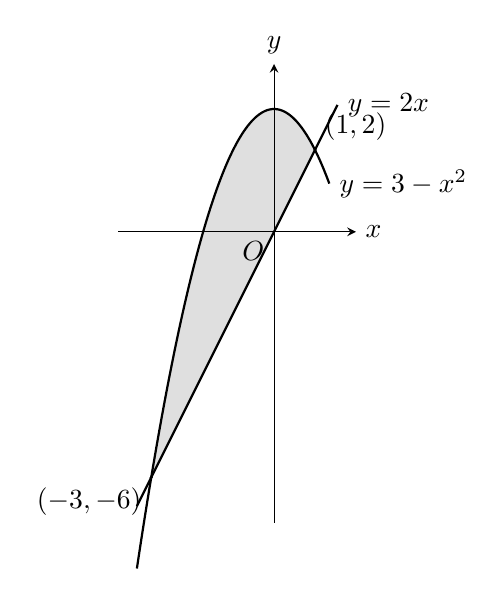
\begin{tikzpicture}[>=stealth, scale=0.52]
  \fill[gray!25]
    (-3,-6) -- plot[domain=-3:1, samples=80] (\x,{3-\x*\x})
    -- (1,2) -- plot[domain=1:-3, samples=20] (\x,{2*\x}) -- cycle;
  \draw[->] (-3.8,0)--(2.0,0) node[right] {$x$};
  \draw[->] (0,-7.1)--(0,4.1) node[above] {$y$};
  \draw[thick, domain=-3.35:1.35, samples=100] plot (\x,{3-\x*\x})
    node[right] {$y=3-x^2$};
  \draw[thick] (-3.35,-6.7)--(1.55,3.1) node[right] {$y=2x$};
  \fill (1,2) circle (1.2pt) node[above right] {$(1,2)$};
  \fill (-3,-6) circle (1.2pt) node[below left] {$(-3,-6)$};
  \node[below left] at (0,0) {$O$};
\end{tikzpicture}
